%##########################################################
\section{Results}
%##########################################################
\label{sec:experiments}

The results are summarized in the following table:

\myorange{build a table, is it worthwhile to use some boxplot?}

Table\ref{tab:tab1} shows the mean and standard deviation of the nonlinear and linear indices computed on healthy and hypoxia cases.

\begin{table*}[t]
\centering
\begin{tabular}{r|ccccc}\hline

	& \textbf{PE}	& \textbf{SampEn}	& \textbf{TI}	& \textbf{STV}	& \textbf{P$_{hf}$}\\
	\hline\hline
{\textbf{Healthy}} & $0.72\pm0.04$ & $0.33\pm0.12$ & $\bm{-0.38\pm0.19^*}$ & $3.23\pm1.15$ &
$0.40\pm0.18$\\
{\textbf{Hypoxia}} & $0.69\pm0.07$ & $0.28\pm0.09$ & $\bm{-0.21\pm0.37}\phantom{*}$ & $3.45\pm1.35$ & $0.43\pm0.25$\\\hline
\end{tabular}
\caption{\emph{Mean$\pm$standard deviation of the nonlinear and linear indices computed on healthy and hypoxia cases. Symbol $^*$ means statistically significant difference (p-value $< 0.1$) using a bootstrap hypothesis test.}}
\label{tab:tab1}
\end{table*}

Entropy indices showed higher complexity (higher values) in healthy fetuses. TI showed values farthest from zero, indicating higher complextiy, in healthy fetuses. Applying the bootstrap hypothesis test we verified a statistical significant difference for TI. 

Figure\ref{} show the box plot for nonlinear indices. 


\begin{figure*}[t]
\centering
\subfigure[]{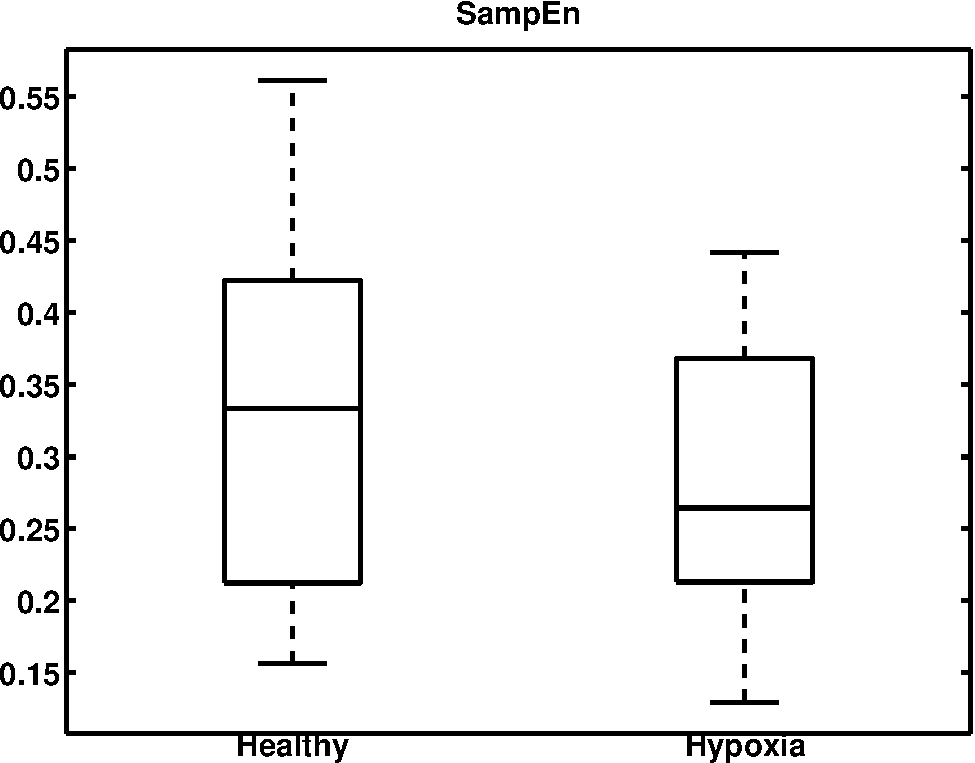
\includegraphics[width=0.35\textwidth]{./figs/sampen_boxplot-crop.pdf}}\\
\subfigure[]{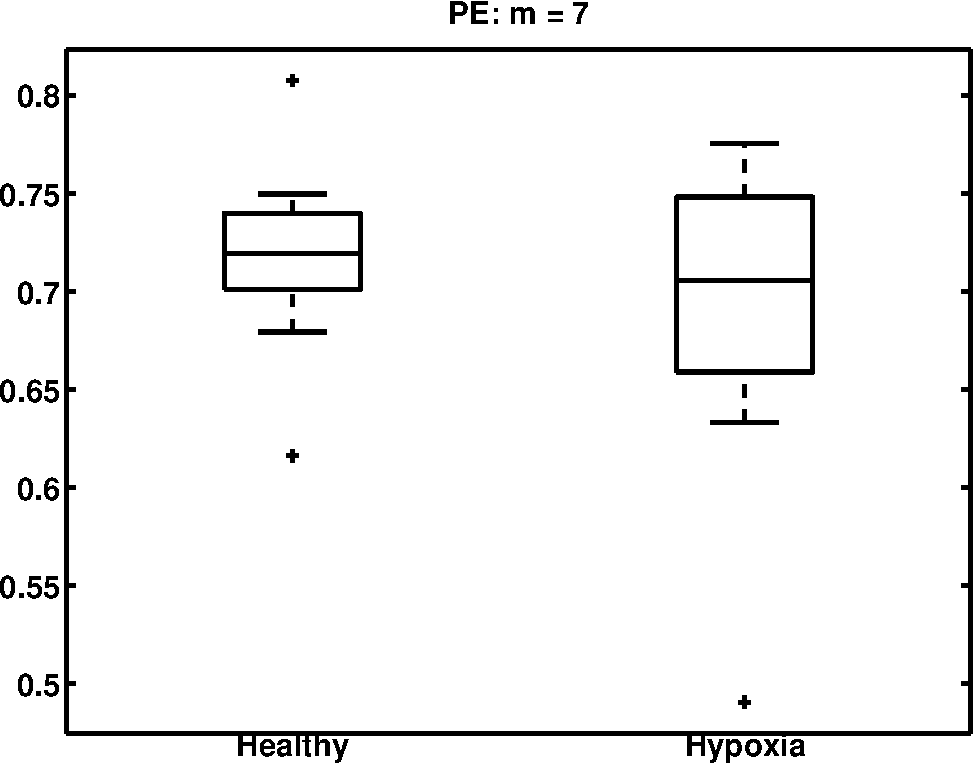
\includegraphics[width=0.35\textwidth]{./figs/pe_fhr-crop.pdf}}
\subfigure[]{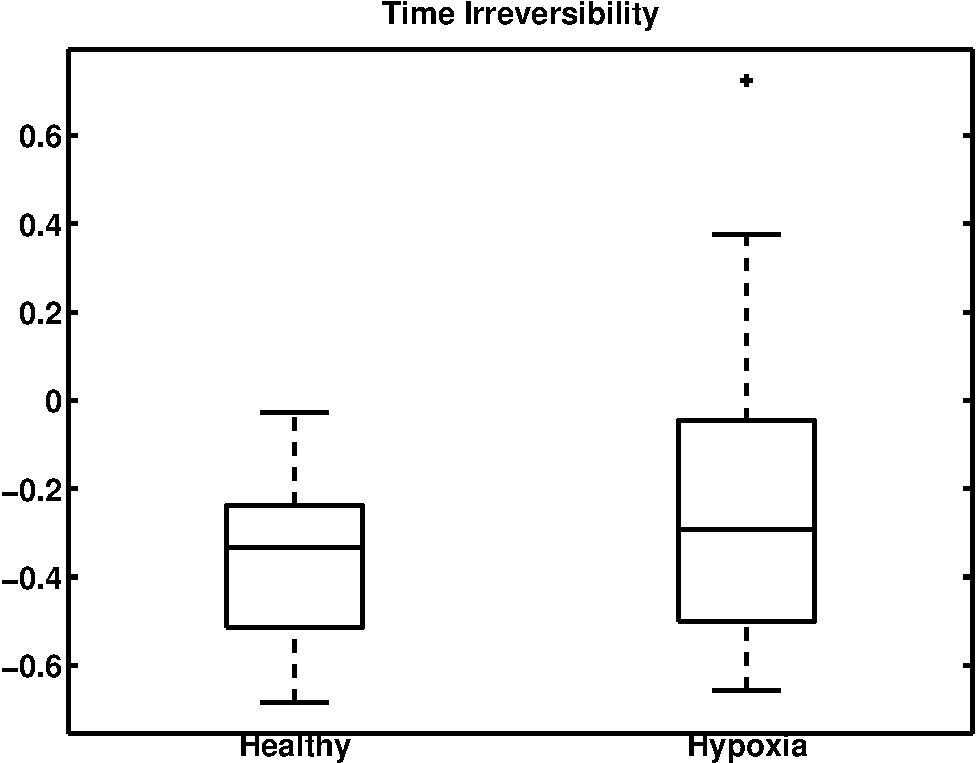
\includegraphics[width=0.35\textwidth]{./figs/ti_fhr-crop.pdf}}\\
\end{figure*}